%\documentclass[11pt,draftcls,onecolumn]{IEEEtran}
\documentclass[10pt,twocolumn]{IEEEtran}

\newcommand{\fv}{\mbox{\boldmath $f$}}
\newcommand{\Iv}{\mbox{\boldmath $I$}}
\newcommand{\xv}{\mbox{\boldmath $x$}}
\newcommand{\velocity}{\mbox{\boldmath $v$}}
\newcommand{\velocityinv}{\mbox{\boldmath $v$}^{-1}}
\newcommand{\Velocityinv}{\mbox{\boldmath $V$}^{-1}}
\newcommand{\Velocity}{\mbox{\boldmath $V$}}
\newcommand{\welocity}{\mbox{\boldmath $w$}}
\newcommand{\spatialimagegradient}{\mbox{\boldmath $I$}\mbox{$_{x}$}}
\newcommand{\perpspatialimagegradient}{\mbox{\boldmath $I$}\mbox{$^{\perp}_{x}$}}
\newcommand{\temporalimagederivative}{\mbox{$I_t$}}
\newcommand{\finitestrain}{\mbox{\boldmath $\varepsilon^{\ast}$}}
\newcommand{\smallstrain}{\mbox{\boldmath $\varepsilon$}}
\newcommand{\dispgradient}{{\bf \nabla \displace}}
\newcommand{\displace}{{\bf u}} 
\newcommand{\Id}{\text{\bf Id}}
\newcommand{\ode}{{\em O.D.E.}}
\newcommand{\odes}{{\em O.D.E.}s}
\newcommand{\G}{\mathcal{G}}
\newcommand{\J}{\mathcal{J}}
\newcommand{\phiinv}{\phi^{-1}}
\newcommand{\psiinv}{\psi^{-1}}
\newcommand{\dM}{DM}
\newcommand{\DM}{Diffeomorphometry}
\newcommand{\diff}{diffeomorphism}
\newcommand{\Diff}{Diffeomorphism}
\newcommand{\orbit}{\mathcal{O}}
\newcommand{\avg}{\mathcal{A}}
\newcommand{\avgn}{\mathcal{A}_n}
\newcommand{\avgna}{\mathcal{A}^a_{n}}
\newcommand{\nset}{\{ J_i \}_n}
\newcommand{\bari}{\bar{I}}
\newcommand{\bart}{\bar{t}}
\newcommand{\jac}{\mathcal{J}}
\newcommand{\pert}{\mbox{\boldmath $w$}}
\newcommand{\barpert}{\bar{\mbox{\boldmath $w$}}}
\newcommand{\half}{0.5}

\newcommand{\X}{{\bf X}}
\newcommand{\x}{{\bf x}}
\newcommand{\Z}{{\bf Z}}
\newcommand{\z}{{\bf z}}
\newcommand{\p}{{\bf p}}
\newcommand{\Y}{{\bf Y}}
\newcommand{\y}{{\bf y}}
\newcommand{\ytild}{\tilde{{\bf y}}}
\newcommand{\q}{{\bf q}}
\newcommand{\surf}{\mathcal{S}}
\newcommand{\phij}{\phi_{ij}}
\newcommand{\aphij}{\bar{\phi}_{j}}
\newcommand{\apsij}{\bar{\psi}_{j}}
\newcommand{\aphi}{\bar{\phi}}
\newcommand{\aphiinv}{\bar{\phi}^{-1}}

\newcommand{\domain}{\Omega}
\newcommand{\meanshape}{\bf \bar{x}}
\newcommand{\g}{\mbox{\boldmath $g$}}
\newcommand{\h}{\mbox{\boldmath $h$}}
\newcommand{\yv}{\mbox{\boldmath $y$}}

\newcommand{\group}{Diff}


\newcommand{\evol}{{E_{\text{Vol}}}}
\newcommand{\epair}{{E_{\text{Pair}}}}
\newcommand{\esec}{{E_{S}}}
\newcommand{\inv}{^{-1}}
\newcommand{\vinit}{ \velocity^0_{ij}(\x,\tau=0) }
\newcommand{\avinit}{ \bar{\velocity}^0_{j}(\x,t) }
\newcommand{\avinitz}{ \bar{\velocity}^0_{j}(\x,t_a) }
\newcommand{\gz}{\nabla_{\z}}

\newcommand{\Section}[1]{\vspace{-8pt}\section{\hskip-1em.~~#1}\vspace{-3pt}}
\newcommand{\SubSection}[1]{\vspace{-3pt}\subsection{\hskip -1em.~~#1}\vspace{-3pt}}

\newcommand{\BASE}{.}%/Users/stnava/Work/}
\newcommand{\TEXDIR}{.}%{\BASE Words/Writing/}
\newcommand{\ROOT}{.}%{\BASE Words/}
\newcommand{\FIGDIR}{.}%{\BASE Words/Writing/MEDIAITK/wbir/}
\newcommand{\FIGDIRAIBS}{.}%{\BASE Words/Writing/IPMI2003/jpegs/}
\newcommand{\FIGDIRP}{proposal/}%{\BASE Words/Writing/proposal/}
\newcommand{\FIGDIRPJ}{proposal/jpegs/}%{\BASE Words/Writing/proposal/jpegs/}
\newcommand{\FIGDIRADAD}{.}%{\BASE Words/Writing/ADAD/}
\newcommand{\FIGS}{.}%{\BASE Words/Writing/neuroimageipam-final/FIGS/}



%% bare_jrnl.tex
%% V1.2
%% 2002/11/18
%% by Michael Shell
%% mshell@ece.gatech.edu
%%
%% NOTE: This text file uses MS Windows line feed conventions. When (human)
%% reading this file on other platforms, you may have to use a text
%% editor that can handle lines terminated by the MS Windows line feed
%% characters (0x0D 0x0A).
%%
%% This is a skeleton file demonstrating the use of IEEEtran.cls
%% (requires IEEEtran.cls version 1.6b or later) with an IEEE journal paper.
%%
%% Support sites:
%% http://www.ieee.org
%% and/or
%% http://www.ctan.org/tex-archive/macros/latex/contrib/supported/IEEEtran/
%%
%% This code is offered as-is - no warranty - user assumes all risk.
%% Free to use, distribute and modify.

% *** Authors should verify (and, if needed, correct) their LaTeX system  ***
% *** with the testflow diagnostic prior to trusting their LaTeX platform ***
% *** with production work. IEEE's font choices can trigger bugs that do  ***
% *** not appear when using other class files.                            ***
% Testflow can be obtained at:
% http://www.ctan.org/tex-archive/macros/latex/contrib/IEEEtran/testflow


% Note that the a4paper option is mainly intended so that authors in
% countries using A4 can easily print to A4 and see how their papers will
% look in print. Authors are encouraged to use U.S. letter paper when 
% submitting to IEEE. Use the testflow package mentioned above to verify
% correct handling of both paper sizes by the author's LaTeX system.
%
% Also note that the "draftcls" or "draftclsnofoot", not "draft", option
% should be used if it is desired that the figures are to be displayed in
% draft mode.
%
% This example can be formatted using the peerreview
% (instead of journal) mode.
%\documentclass[11pt,draftcls,onecolumn]{IEEEtran}
\usepackage{amssymb,amsmath}
\usepackage{color}
\usepackage{algorithm}
\usepackage{algorithmic}
\usepackage{rotating}
\usepackage{multirow,booktabs,ctable,array}
\usepackage{listing}						
\usepackage{listings}					
\graphicspath{./Figures/}



% If the IEEEtran.cls has not been installed into the LaTeX system files,
% manually specify the path to it:
% \documentclass[journal]{../sty/IEEEtran}


% some very useful LaTeX packages include:

%\usepackage{cite}      % Written by Donald Arseneau
                        % V1.6 and later of IEEEtran pre-defines the format
                        % of the cite.sty package \cite{} output to follow
                        % that of IEEE. Loading the cite package will
                        % result in citation numbers being automatically
                        % sorted and properly "ranged". i.e.,
                        % [1], [9], [2], [7], [5], [6]
                        % (without using cite.sty)
                        % will become:
                        % [1], [2], [5]--[7], [9] (using cite.sty)
                        % cite.sty's \cite will automatically add leading
                        % space, if needed. Use cite.sty's noadjust option
                        % (cite.sty V3.8 and later) if you want to turn this
                        % off. cite.sty is already installed on most LaTeX
                        % systems. The latest version can be obtained at:
                        % http://www.ctan.org/tex-archive/macros/latex/contrib/supported/cite/

%\usepackage{graphicx}  % Written by David Carlisle and Sebastian Rahtz
                        % Required if you want graphics, photos, etc.
                        % graphicx.sty is already installed on most LaTeX
                        % systems. The latest version and documentation can
                        % be obtained at:
                        % http://www.ctan.org/tex-archive/macros/latex/required/graphics/
                        % Another good source of documentation is "Using
                        % Imported Graphics in LaTeX2e" by Keith Reckdahl
                        % which can be found as esplatex.ps and epslatex.pdf
                        % at: http://www.ctan.org/tex-archive/info/
% NOTE: for dual use with latex and pdflatex, instead load graphicx like:
%\ifx\pdfoutput\undefined
%\usepackage{graphicx}
%\else
%\usepackage[pdftex]{graphicx}
%\fi

% However, be warned that pdflatex will require graphics to be in PDF
% (not EPS) format and will preclude the use of PostScript based LaTeX
% packages such as psfrag.sty and pstricks.sty. IEEE conferences typically
% allow PDF graphics (and hence pdfLaTeX). However, IEEE journals do not
% (yet) allow image formats other than EPS or TIFF. Therefore, authors of
% journal papers should use traditional LaTeX with EPS graphics.
%
% The path(s) to the graphics files can also be declared: e.g.,
% \graphicspath{{../eps/}{../ps/}}
% if the graphics files are not located in the same directory as the
% .tex file. This can be done in each branch of the conditional above
% (after graphicx is loaded) to handle the EPS and PDF cases separately.
% In this way, full path information will not have to be specified in
% each \includegraphics command.
%
% Note that, when switching from latex to pdflatex and vice-versa, the new
% compiler will have to be run twice to clear some warnings.


%\usepackage{psfrag}    % Written by Craig Barratt, Michael C. Grant,
                        % and David Carlisle
                        % This package allows you to substitute LaTeX
                        % commands for text in imported EPS graphic files.
                        % In this way, LaTeX symbols can be placed into
                        % graphics that have been generated by other
                        % applications. You must use latex->dvips->ps2pdf
                        % workflow (not direct pdf output from pdflatex) if
                        % you wish to use this capability because it works
                        % via some PostScript tricks. Alternatively, the
                        % graphics could be processed as separate files via
                        % psfrag and dvips, then converted to PDF for
                        % inclusion in the main file which uses pdflatex.
                        % Docs are in "The PSfrag System" by Michael C. Grant
                        % and David Carlisle. There is also some information 
                        % about using psfrag in "Using Imported Graphics in
                        % LaTeX2e" by Keith Reckdahl which documents the
                        % graphicx package (see above). The psfrag package
                        % and documentation can be obtained at:
                        % http://www.ctan.org/tex-archive/macros/latex/contrib/supported/psfrag/

%\usepackage{subfigure} % Written by Steven Douglas Cochran
                        % This package makes it easy to put subfigures
                        % in your figures. i.e., "figure 1a and 1b"
                        % Docs are in "Using Imported Graphics in LaTeX2e"
                        % by Keith Reckdahl which also documents the graphicx
                        % package (see above). subfigure.sty is already
                        % installed on most LaTeX systems. The latest version
                        % and documentation can be obtained at:
                        % http://www.ctan.org/tex-archive/macros/latex/contrib/supported/subfigure/

%\usepackage{url}       % Written by Donald Arseneau
                        % Provides better support for handling and breaking
                        % URLs. url.sty is already installed on most LaTeX
                        % systems. The latest version can be obtained at:
                        % http://www.ctan.org/tex-archive/macros/latex/contrib/other/misc/
                        % Read the url.sty source comments for usage information.

%\usepackage{stfloats}  % Written by Sigitas Tolusis
                        % Gives LaTeX2e the ability to do double column
                        % floats at the bottom of the page as well as the top.
                        % (e.g., "\begin{figure*}[!b]" is not normally
                        % possible in LaTeX2e). This is an invasive package
                        % which rewrites many portions of the LaTeX2e output
                        % routines. It may not work with other packages that
                        % modify the LaTeX2e output routine and/or with other
                        % versions of LaTeX. The latest version and
                        % documentation can be obtained at:
                        % http://www.ctan.org/tex-archive/macros/latex/contrib/supported/sttools/
                        % Documentation is contained in the stfloats.sty
                        % comments as well as in the presfull.pdf file.
                        % Do not use the stfloats baselinefloat ability as
                        % IEEE does not allow \baselineskip to stretch.
                        % Authors submitting work to the IEEE should note
                        % that IEEE rarely uses double column equations and
                        % that authors should try to avoid such use.
                        % Do not be tempted to use the cuted.sty or
                        % midfloat.sty package (by the same author) as IEEE
                        % does not format its papers in such ways.

%\usepackage{amsmath}   % From the American Mathematical Society
                        % A popular package that provides many helpful commands
                        % for dealing with mathematics. Note that the AMSmath
                        % package sets \interdisplaylinepenalty to 10000 thus
                        % preventing page breaks from occurring within multiline
                        % equations. Use:
%\interdisplaylinepenalty=2500
                        % after loading amsmath to restore such page breaks
                        % as IEEEtran.cls normally does. amsmath.sty is already
                        % installed on most LaTeX systems. The latest version
                        % and documentation can be obtained at:
                        % http://www.ctan.org/tex-archive/macros/latex/required/amslatex/math/



% Other popular packages for formatting tables and equations include:

%\usepackage{array}
% Frank Mittelbach's and David Carlisle's array.sty which improves the
% LaTeX2e array and tabular environments to provide better appearances and
% additional user controls. array.sty is already installed on most systems.
% The latest version and documentation can be obtained at:
% http://www.ctan.org/tex-archive/macros/latex/required/tools/

% Mark Wooding's extremely powerful MDW tools, especially mdwmath.sty and
% mdwtab.sty which are used to format equations and tables, respectively.
% The MDWtools set is already installed on most LaTeX systems. The lastest
% version and documentation is available at:
% http://www.ctan.org/tex-archive/macros/latex/contrib/supported/mdwtools/


% V1.6 of IEEEtran contains the IEEEeqnarray family of commands that can
% be used to generate multiline equations as well as matrices, tables, etc.


% Also of notable interest:

% Scott Pakin's eqparbox package for creating (automatically sized) equal
% width boxes. Available:
% http://www.ctan.org/tex-archive/macros/latex/contrib/supported/eqparbox/



% Notes on hyperref:
% IEEEtran.cls attempts to be compliant with the hyperref package, written
% by Heiko Oberdiek and Sebastian Rahtz, which provides hyperlinks within
% a document as well as an index for PDF files (produced via pdflatex).
% However, it is a tad difficult to properly interface LaTeX classes and
% packages with this (necessarily) complex and invasive package. It is
% recommended that hyperref not be used for work that is to be submitted
% to the IEEE. Users who wish to use hyperref *must* ensure that their
% hyperref version is 6.72u or later *and* IEEEtran.cls is version 1.6b
% or later. The latest version of hyperref can be obtained at:
%
% http://www.ctan.org/tex-archive/macros/latex/contrib/supported/hyperref/
%
% Also, be aware that cite.sty (as of version 3.9, 11/2001) and hyperref.sty
% (as of version 6.72t, 2002/07/25) do not work optimally together.
% To mediate the differences between these two packages, IEEEtran.cls, as
% of v1.6b, predefines a command that fools hyperref into thinking that
% the natbib package is being used - causing it not to modify the existing
% citation commands, and allowing cite.sty to operate as normal. However,
% as a result, citation numbers will not be hyperlinked. Another side effect
% of this approach is that the natbib.sty package will not properly load
% under IEEEtran.cls. However, current versions of natbib are not capable
% of compressing and sorting citation numbers in IEEE's style - so this
% should not be an issue. If, for some strange reason, the user wants to
% load natbib.sty under IEEEtran.cls, the following code must be placed
% before natbib.sty can be loaded:
%
% \makeatletter
% \let\NAT@parse\undefined
% \makeatother
%
% Hyperref should be loaded differently depending on whether pdflatex
% or traditional latex is being used:
%
%\ifx\pdfoutput\undefined
%\usepackage[hypertex]{hyperref}
%\else
%\usepackage[pdftex,hypertexnames=false]{hyperref}
%\fi
%
% Pdflatex produces superior hyperref results and is the recommended
% compiler for such use.



% *** Do not adjust lengths that control margins, column widths, etc. ***
% *** Do not use packages that alter fonts (such as pslatex).         ***
% There should be no need to do such things with IEEEtran.cls V1.6 and later.


% correct bad hyphenation here
\hyphenation{op-tical net-works semi-conduc-tor}


% The lineno packages adds line numbers. Start line numbering with
% \begin{linenumbers}, end it with \end{linenumbers}. Or switch it on
% for the whole article with \linenumbers.
 \usepackage{lineno}

%\linenumbers
\begin{document}


%Setup listing environment
\definecolor{listcomment}{rgb}{0.0,0.5,0.0}
\definecolor{listkeyword}{rgb}{0.0,0.0,0.5}
\definecolor{listbackground}{gray}{0.965}

\lstset{frame = tb,
        framerule = 0.25pt,
        float,
        fontadjust,
        backgroundcolor={\color{listbackground}},
        basicstyle = {\ttfamily\scriptsize},
        keywordstyle = {\ttfamily\color{listkeyword}\textbf},
        identifierstyle = {\ttfamily},
        commentstyle = {\ttfamily\color{listcomment}\textit},
        stringstyle = {\ttfamily},
        showstringspaces = false,
        showtabs = false,
        numbers = none,
        tabsize = 2,
        language=[ISO]C++,
        floatplacement=!h
        }	



%
% paper title
\title{ANTS:  Advanced Open-Source Tools for Normalization And Neuroanatomy}
%
%
% author names and IEEE memberships
% note positions of commas and nonbreaking spaces ( ~ ) LaTeX will not break
% a structure at a ~ so this keeps an author's name from being broken across
% two lines.
% use \thanks{} to gain access to the first footnote area
% a separate \thanks must be used for each paragraph as LaTeX2e's \thanks
% was not built to handle multiple paragraphs
\author{Brian B. Avants, Nicholas J. Tustison, Gang Song, and James C. Gee
%               Penn Image Computing and Science Laboratory \\
%               University of Pennsylvania \\
%               3600 Market Street, Suite 370 \\
%               Philadelphia,  PA  19104 \\
%               contact email:  tustison@grasp.cis.upenn.edu
%\thanks{Manuscript received XXX; revised XXX.
 %       }% <-this % stops a space
}

% note the % following the last \IEEEmembership and also the first \thanks - 
% these prevent an unwanted space from occurring between the last author name
% and the end of the author line. i.e., if you had this:
% 
% \author{....lastname \thanks{...} \thanks{...} }
%                     ^------------^------------^----Do not want these spaces!
%
% a space would be appended to the last name and could cause every name on that
% line to be shifted left slightly. This is one of those "LaTeX things". For
% instance, "A\textbf{} \textbf{}B" will typeset as "A B" not "AB". If you want
% "AB" then you have to do: "A\textbf{}\textbf{}B"
% \thanks is no different in this regard, so shield the last } of each \thanks
% that ends a line with a % and do not let a space in before the next \thanks.
% Spaces after \IEEEmembership other than the last one are OK (and needed) as
% you are supposed to have spaces between the names. For what it is worth,
% this is a minor point as most people would not even notice if the said evil
% space somehow managed to creep in.
%
% The paper headers
\markboth{IEEE Transactions on Medical Imaging,~Vol.~X, No.~XX,~November~200X}{Tustison\MakeLowercase{\textit{et al.}}: Advanced Normalization Tools}
% The only time the second header will appear is for the odd numbered pages
% after the title page when using the twoside option.
% 
% *** Note that you probably will NOT want to include the author's name in ***
% *** the headers of peer review papers.                                   ***

% If you want to put a publisher's ID mark on the page
% (can leave text blank if you just want to see how the
% text height on the first page will be reduced by IEEE)
%\pubid{0000--0000/00\$00.00~\copyright~2002 IEEE}

% use only for invited papers
%\specialpapernotice{(Invited Paper)}

% make the title area

\maketitle

\begin{abstract}
Computational anatomy (CA) seeks to quantify natural variation in
biological shape and function with roots that reach back to the
seminal works of Charles Darwin and D'arcy Thompson.  CA is currently
applied to study health, disease and epidemiology and uses deformable
mappings between images as a basic technique.  However, there is a
lack of standards and reproducibility in the field that is due, in
part, to the use of proprietary software and private data.  To
facilitate reproducibility in CA measurements and advancement of
imaging sciences, NIH has recently committed significant support to
open-source data and software resources.  Here, we report a recent
product of this commitment: Advanced Normalization Tools (ANTS), an
ITK-based toolkit for CA and related areas.  The ANTS open-source
library consists of a well-evaluated suite of state-of-the-art
normalization and template-building tools for quantitative
morphometric analysis.  We highlight the prominent features of ANTS
and demonstrate its utility by performing a detailed analysis on
openly-available anatomically labeled brain data from the non-rigid
image registration evaluation project (NIREP).  The results from this
analysis evidences the high level of accuracy achievable with ANTS
using intensity-based registration alone.  In addition, we show the
significant performance gains may be achieved by coupling
intensity-based image metrics and point-set-based metrics from
specific, sensibly selected cortical structures.
%Computational anatomy is the quantitative study of biological shape and its natural variations which traces its roots to the seminal works of Charles Darwin and D'arcy Thompson.  Integral to this research field is the calculation of deformable mappings between images that serve as invaluable measurement tools.  Technological evolution has spawned much innovation in the computational development of such deformable mapping algorithms.  However, not only is algorithmic development essential for increasing scientific knowledge but the availability of these technologies is equally crucial for facilitating the progress of the scientific community at large.  This is the motivation behind such projects as the Insight Toolkit (ITK) of the National Institutes of Health which serves as a repository for many popular image segmentation and registration routines.  In addition, the ITK library provides a well-structured framework for several stand-alone projects such as Elastix, ITK-SNAP, ManagedITK, the Medical Imaging Toolkit (MITK), WrapITK, and many others.  Our own  contribution to the field of computational anatomy, also built on an ITK foundation, is called Advanced Normalization Tools (ANTS).  The ANTS open-source library consists of an entire suite of state-of-the-art normalization and template-building tools for quantitative morphometric analysis. After highlighting the prominent features of ANTS, we demonstrate its utility by performing a detailed analysis on anatomically labeled brain data from the non-rigid image registration evaluation project (NIREP).  The results from this analysis evidences the high level of accuracy achievable with ANTS using intensity-based registration alone.  In addition, we show the performance gains achieved by coupling intensity-based image metrics and point-set-based metrics from specific, sensibly selected cortical structures.
  
%In a recent evaluation of 14 non-linear deformation algorithms \cite{Klein2009}, the SyN algorithm of ANTS was consistently one of the top performers.

\end{abstract}

\IEEEkeywords{
ANTS, image registration, nueroanatomy, neuroimaging, normalization, open-source, point-set registration
}

\IEEEpeerreviewmaketitle

\section{Introduction}

The rapid advancement of biological and medical imaging technologies has caused a proliferation in the development of quantitative tools for computational anatomy.  The principal tools of this emerging field are meaningful deformable mappings between images whether they be driven by similarity metrics which are intensity-based,  point-set based, or both.  Several categories of mappings have been proposed in the literature.  Of particular recent interest are diffeomorphic transformations which, by definition, preserve topology.  Topology preservation is fundamental to making comparisons between objects in the natural world as such transformations permit comparisons to be made across time points in an individual's disease process or to study development patterns across a large population.

Despite the number of proposed algorithms, our limited assessment of published research mirrors the experience of many others who prefer a working paradigm of what has been referred to as {\em reproducible research}.  As described by Dr. Kovacevic ``[reproducible research] refers to the idea that, in `computational' sciences, the ultimate product is not a published paper but, rather, the entire environment used to produce the results in the paper (data, software,etc.).''  After an informal survey of 15 published papers, she found ``none had code available'' and ``in only about half the cases were the parameters [of the algorithm] specified'' \cite{Kovacevic2006}.  Recent discussions within the computational sciences research community, particularly among advocates of ``open science,'' have also voiced similar concerns \cite{Yoo2005,Ibanez2006}.   In this paper, we discuss our contribution to the open-source medical image analysis research community which we call ANTS (\underline{A}dvanced \underline{N}ormalization \underline{T}ool\underline{s}).  Built on an ITK framework, this software package comprises a suite of tools for image normalization and template building based on previously published research.  

 
Perhaps the most persuasive evidence motivating the use of our contributions discussed in this paper is the recent outcome of a large-scale comparative image registration algorithm assessment \cite{Klein2009}. In the largest evaluation study to date involving 14 popular non-linear registration algorithms, our Symmetric Normalization (SyN) transformation model \cite{Avants2008} discussed below, was consistently one of the top two performers across all tests.  Overlap and distance measures used for assessment employed three completely independent analysis methods (permutation tests, one-way ANOVA tests, and indifference zone ranking).  Unlike some of the other algorithms used in this brain registration evaluation study, all of our methods (not just SyN) are available as open-source.  

We first provide an overview of the different components included in ANTS, such as the available transformation models and similarity metrics offered.  This is followed by an extensive experimental analysis that builds upon the results from the recent image normalization evaluation of \cite{Klein2009} which was limited to a single configuration of ANTS.  This will provide  a useful benchmark for evaluating other possible ANTS configurations.

\section{Theoretical Overview of ANTS}
A useful classification schema of normalization techniques is based upon the following three principal components \cite{Brown1992,Ibanez2002}:
\begin{itemize}
  \item the {\em transformation model},
  \item the {\em similarity (or correspondence) measures},  and
  \item the {\em optimization strategy}.
\end{itemize}
In general, image normalization is the process of finding the optimal transformation, $\phi$, within a specified transformation space which maps each $\mathbf{x}$ of image $\mathcal{I}(\mathbf{x})$ to a location in image $\mathcal{J}(\mathbf{z})$ such that a specified cost function, $\mathcal{C}$, describing the similarity between $\mathcal{I}$ and $\mathcal{J}$, is minimized.   A summary of available transformation models and similarity measures are provided in Table \ref{table:chart}.  Details are given in subsequent sections.

\subsection{ANTS Transformation Models}

%\begin{figure*}
%  \centering
%    \begin{tabular}{c}
%      \includegraphics[width=170mm]{TransformationTable}
%    \end{tabular}
%  \caption{Available transformations and similarity metrics available in ANTS.  Similarity metric acronyms:  CC = cross correlation, MSQ = mean squares, MI = mutual information, JHCT = Jensen-Havrda-Charvat-Tsallis divergence, PSE = point-set expectation.  }
%  \label{fig:chart}
%\end{figure*}

\begin{table*}
  \centering
    \begin{tabular}{c c c c}
    {\bf Category} & {\bf Transformation, $\phi$} & {\bf Similarity Measures} & {\bf Brief Description} \\
    \toprule     
    \multirow{2}*{\bf Linear}
           & Rigid$^\dagger$ & MI, MSQ & translation and rotation \\
       {} & Affine$^\dagger$ & MI, MSQ & rigid, scaling, and shear \\
       \cmidrule(l){2-4}
    \multirow{2}*{\bf Elastic}
           & Deformable & CC, PR, MI, MSQ, JHCT, PSE & Demons-like algorithm \\
       {} & DMFFD & CC, PR, MI, MSQ, JHCT, PSE  & FFD variant \\
       \cmidrule(l){2-4}
    \multirow{2}*{\bf Diffeomorphic}
           & Exponential &  CC,PR, MI, MSQ, JHCT, PSE  & minimizes $\boldsymbol{v}(\mathbf{x})$ \\
       {} & Greedy SyN$^\dagger$ &  CC, PR, MI, MSQ, JHCT, PSE  & minimizes $\boldsymbol{v}(\mathbf{x,t})$ locally in time \\
       {} & Geodesic SyN$^\dagger$ &  CC, PR, MI, MSQ, JHCT, PSE  & minimizes $\boldsymbol{v}(\mathbf{x,t})$ over all time \\
    \bottomrule
    \end{tabular}
  \caption{Available transformations and similarity metrics available in ANTS.  Similarity metric acronyms:  CC = cross correlation, PR = probabilistic matching, MSQ = mean squared difference, MI = mutual information, JHCT = Jensen-Havrda-Charvat-Tsallis divergence, PSE = point-set expectation.  ANTS also provides the inverse of those transformations denoted by the `$\dagger$' symbol.}
  \label{table:chart}
\end{table*}    


A variety of transformation models have been proposed in the literature with varying degrees of freedom (illustrated in Figure \ref{fig:hierarchy}).  For deformable transformations, one approach is to optimize within the space of non-topology preserving, yet physically motivated transformations---an approach pioneered by Bajcsy \cite{Bajcsy1989}.  Elastic and related models, such as HAMMER \cite{Shen2002}, statistical parametric mapping (SPM) \cite{Ashburner2000}, free-form deformations (FFD) \cite{Rueckert1999}, and
Thirion's demons \cite{Thirion1998} operate in the space of vector fields, which does not preserve topology.  In other words, barring ad hoc constraints to prevent otherwise, these algorithms allow the topology to change in an uncontrolled way which makes the deformable mappings difficult to interpret in functional or anatomical studies.   

These topology concerns have led to current advocation within the computational anatomy research community of diffeomorphic mappings for transformation modeling.   Optimizing directly within this space has shown remarkable success in various computational anatomy studies involving longitudinal \cite{Avants2007b,Fox2001}, functional \cite{Miller2005}, and population data \cite{Avants2007b}.  We include three such diffeomorphic algorithms in the ANTS toolbox based on previously reported research.

Regardless of current research trends, however, we recognize that selection of the transformation model is ultimately application-specific, that no single choice is optimal for all scenarios \cite{Wolpert1997}, and, therefore, the transformation model must be chosen in a principled fashion.  In fact, several non-diffeomorphic algorithms performed quite well in Klein's comparative study of nonrigid registration algorithms \cite{Klein2009}.  For this reason, we also include elastic-related methods for a panoply of transformation model options. 

\begin{figure}
  \centering
    \begin{tabular}{c}
      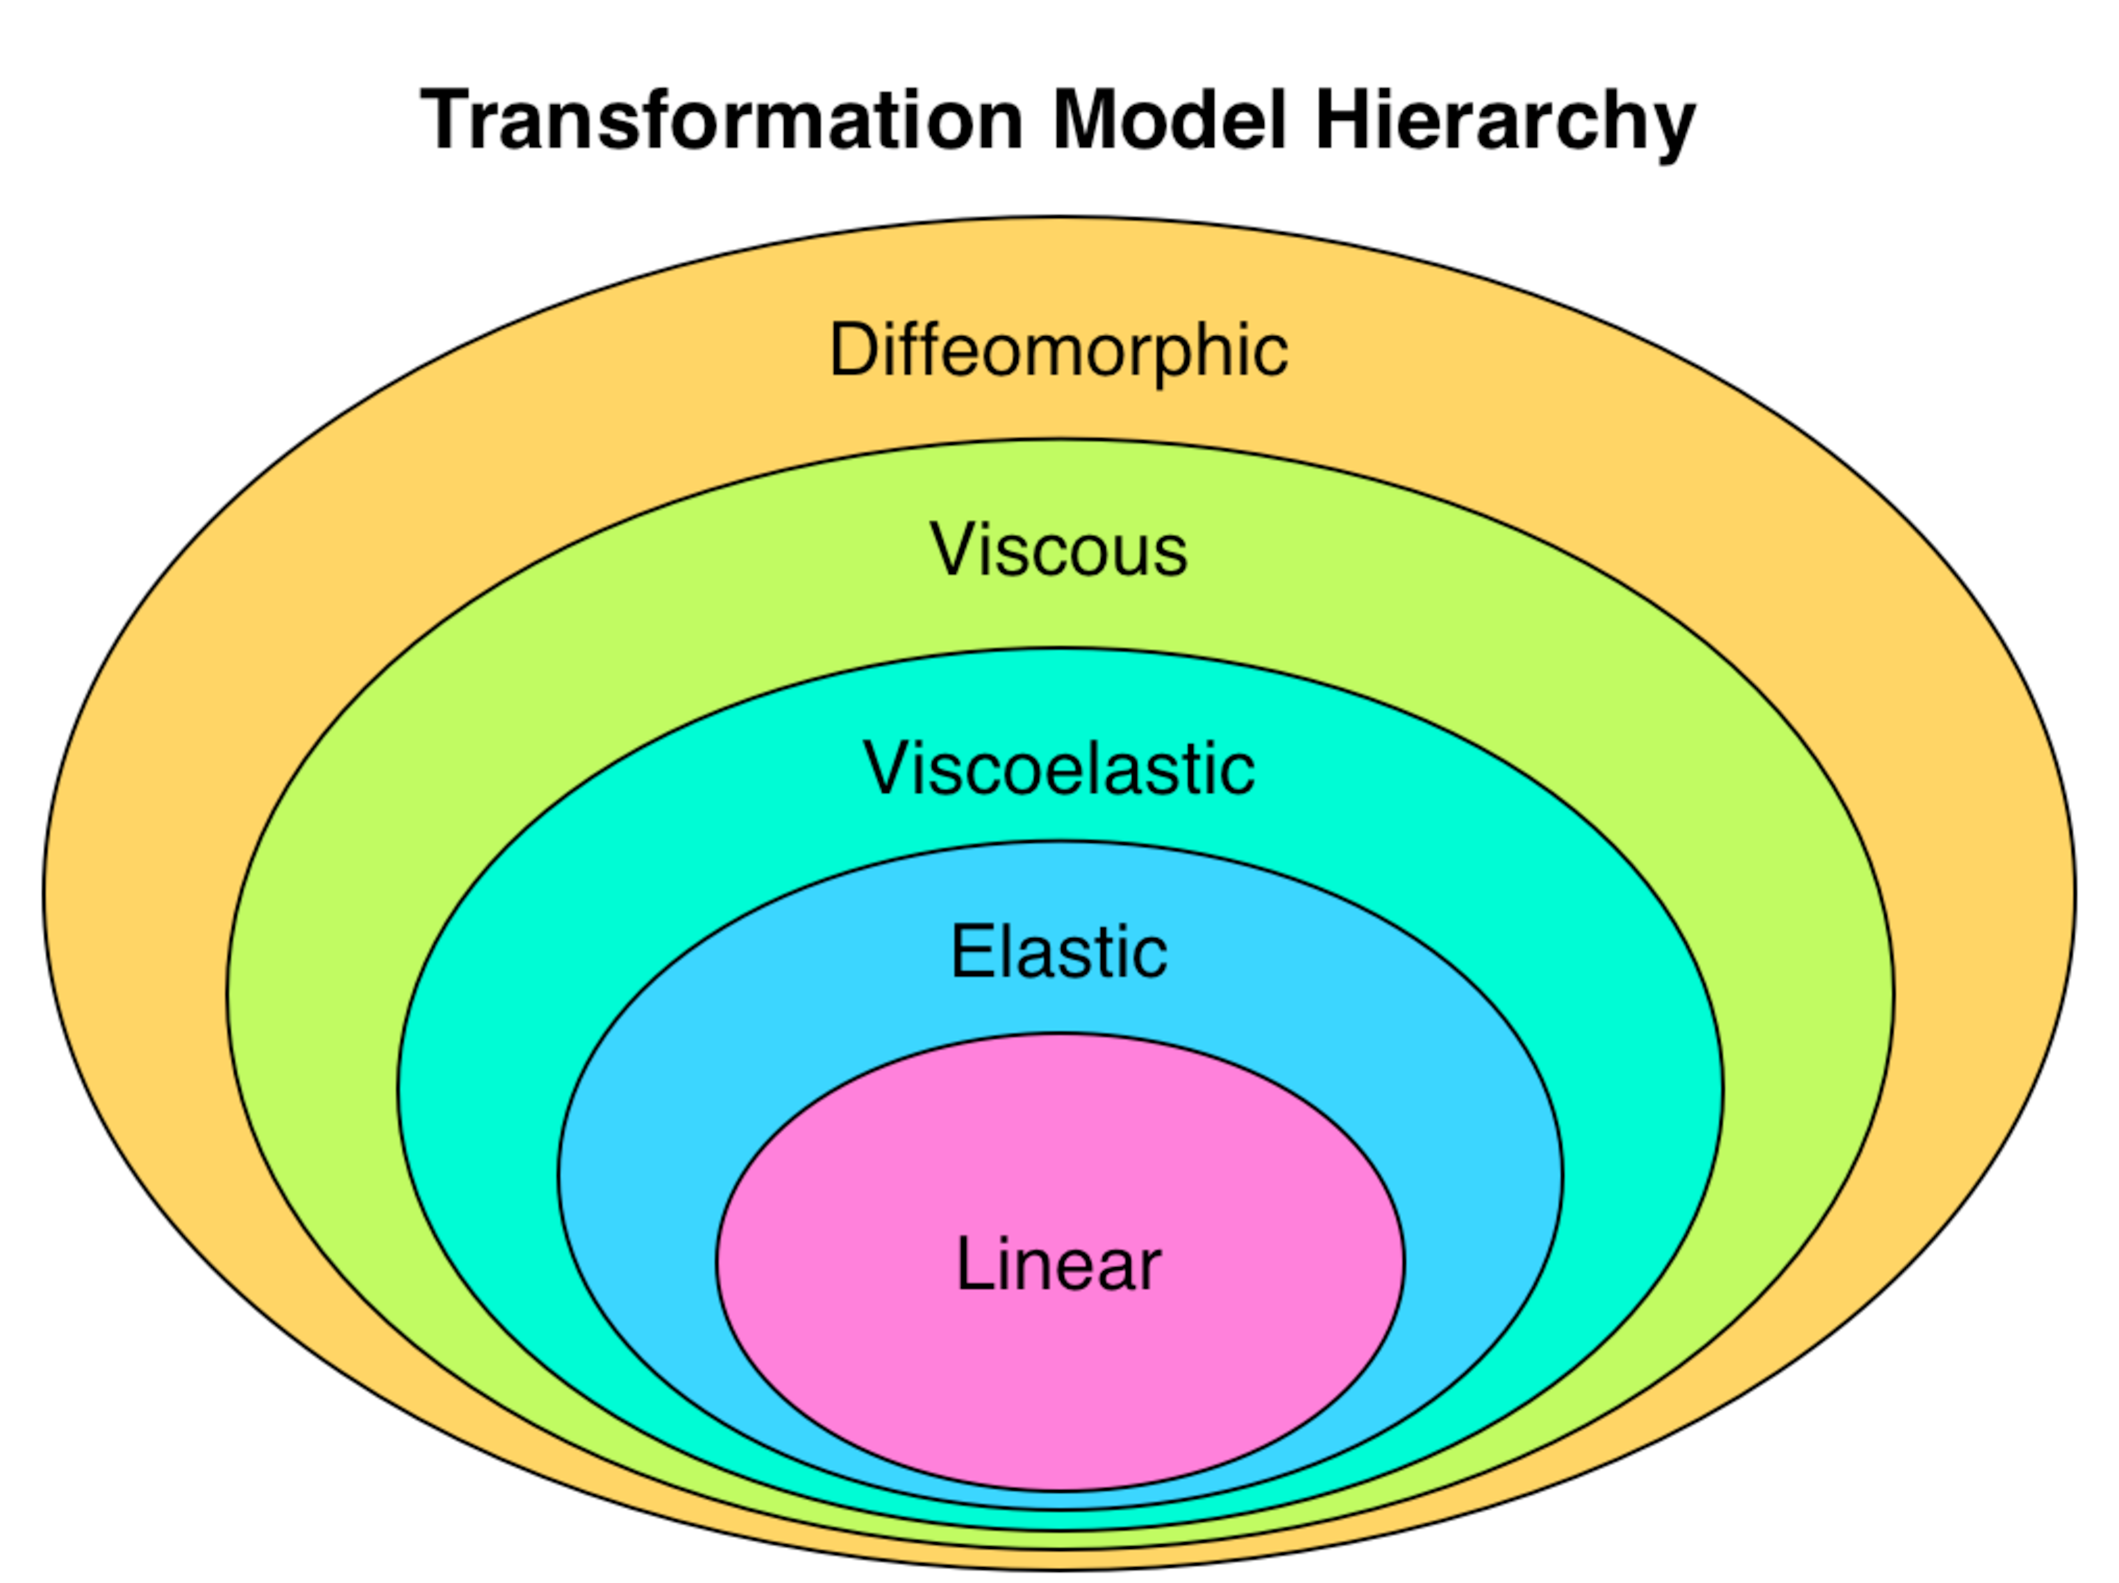
\includegraphics[width=80mm]{Figures/hierarchy}
    \end{tabular}
  \caption{Diagrammatic illustration of the transformation model hierarchy where the encompassing transformation spaces are characterized by increasing degrees of freedom.  }
  \label{fig:hierarchy}
\end{figure}



\subsubsection{Rigid and Affine Linear Transformations }

Image registration strategies often begin with a linear transformation for initial global alignment which precedes a deformable transformation with increased degrees of freedom.  The linear transformations available within ANTS optimize either a mean-squared difference (MSQ) or mutual information (MI) similarity metric which are optimized with respect to translation, rotation, and, in the case of affine transformations, scaling and shearing.  The successive optimization of each component of the linear transformation allows for careful control over increasing degrees of freedom.   ANTS also composes the affine transformation with the deformable transformation field before performing any interpolation or downsampling.  In this way, ANTS normalization never requires more than a single image interpolation step and is able to always refer back to the original full-resolution image sources.    
%We have implemented quaternion-based rigid and affine transformations within ANTS.  Not only does this facilitate accessibility of a sound global alignment strategy, but the parameters of the calculated optimal linear transformation can be maintained internally to ANTS to avoid unnecessary image interpolations.  Either a mean-squared difference metric or a mutual information metric can be used for the linear alignment.

\subsubsection{Vector Field Operators for Regularization} Antecedent to discussion of available deformable transformation models, we point out that  deformable normalization strategies typically invoke a deformation regularization step which smooths the displacement field, $\displace$, or velocity field, $\mathbf{v}$,  or both by a linear operator such as the Laplacian or Navier-Stokes operator. One may write this regularization as a variational minimization in terms of its linear operator or in
terms of a kernel function operating of the field itself, e.g., $
\displace_{smooth}= K \star \displace_{not \,\, smooth}$, where $K \star$ denotes 
convolution with the Green's kernel, $K$, for the linear operator, $L$.  


Regularization models operate on either the
whole mapping $\phi$ or the gradient of the similarity term or both.
The same regularization schema is available for both diffeomorphic and the recently 
proposed directly manipulated free-form deformation
(DMFFD) \cite{Tustison2009}, allowing regularization of both total 
deformation and deformation update.  Viewed from this perspective, hybrid configurations incorporating discretized FFD strategies and diffeomorphisms can be combined for novel 
image normalization approaches.

ANTS enables a variety of choices for $K$
including the Gaussian with varying $\sigma$ and a variety of B-spline
functions, both of which induce adequate regularity for normalization
models used in ANTS.  While additional physical operators will be
included in future releases, current B-spline options provide many orders 
of flexibility \cite{Tustison2005}.

\subsubsection{Diffeomorphic Transformations}

In contrast to many transformation models which reside in the domain of vector spaces, a diffeomorphism is a differentiable mapping with a differentiable inverse \cite{Ebin1970,Mumford1998}.  Modeling transformations with diffeomorphisms ensures certain desirable topological properties that cannot be guaranteed with other methods.  

ANTS assumes the diffeomorphism, $\phi$, is defined on the image domain, $\Omega$, an maintains an affine transform at the boundary such that $\phi(\partial \Omega) = A(\mathbf{Id})$ where $A(\mathbf{Id})$ is an affine mapping applied to the identity transformation.  $\phi$, over time, parameterizes a family of diffeomorphisms, $\phi(\mathbf{x}, t) : \Omega \times t \rightarrow  \Omega$, which can be generated by integrating a time-dependent, smooth velocity field, $\boldsymbol{v} : \Omega \times t \rightarrow \mathbb{R}^d$,  through the ordinary differential equation (o.d.e.)
\begin{align} \label{eq:ode}
\frac{d \phi(\mathbf{x}, t)}{dt} = \boldsymbol{v}(\phi(\mathbf{x}, t), t), \,\,\, \phi(\mathbf{x}, 0) = \mathbf{x}.
\end{align}
The existence and uniqueness theorem for o.d.e.'s implies that integrating Equation (\ref{eq:ode}) generates a diffeomorphism.  The deformation field yielded by $\phi$ is $\mathbf{u}(\mathbf{x}) = \phi(\mathbf{x},1) - \mathbf{x}$.

Dupuis et al. \cite{Dupuis1998} motivated the usage of diffeomorphisms for CA  by showing that the variational form
\begin{align}\label{eq:D}
  D(\mathcal{I}, \mathcal{J}) =  \int_0^1 ||L\boldsymbol{v}||^2 dt , \,\, \mathcal{I}(\phi(\mathbf{x}, 1)) = \mathcal{J}(\mathbf{z})
\end{align}
represents a true mathematical metric between anatomical instances $\mathcal{I}$ and $\mathcal{J}$ given an appropriate norm, $L$, on the velocity field, $\boldsymbol{v}$.  An optimal solution, $\boldsymbol{v}^*$, minimizes the metric $D(\mathcal{I}, \mathcal{J})$ with respect to $L$.   Dupuis \cite{Dupuis1998} also showed that such a solution is guaranteed to be well-posed.  Intuitively, Equation (\ref{eq:D}) provides a sense of distance between two anatomical shapes.  It also illustrates that the optimal diffeomorphic solution is analogous to finding the geodesic curve between two points in a curved space.%
\footnote{
It is important to note the similarity between the definition of curve length, $\int ||\mathcal{C}'(t)||dt$, for the parametric curve $\mathcal{C}(t)$ and Equation (\ref{eq:D}).  In this sense, the solution for Equation (\ref{eq:D}) is the geodesic diffeomorphism, where $\boldsymbol{v}$ is the tangent vector of the diffeomorphism, such that the shape distance, $D$, between $\mathcal{I}$ and $\mathcal{J}$ is minimized.
}

In most real-world applications, however, a diffeomorphic path connecting the anatomical instance $\mathcal{J}$ with $\mathcal{I}$ is non-existent (due, for example, to the photometric variation or the presence/absence of a tumor in neuroanatomical images).  Therefore, the following minimizing variational form is used for optimization in diffeomorphic normalization to accommodate inexact matching  \cite{Dupuis1998,Miller2002}
\begin{align} \label{eq:lddmm}
  \boldsymbol{v}^* = \underset{\boldsymbol{v}}{\operatorname{argmin}}  \left\{ \int_0^1  ||L\boldsymbol{v}||^2dt  + \lambda\int_{\Omega} || \mathcal{I} \circ \phi(\mathbf{x},1) - \mathcal{J}  || d\Omega \right\}.
\end{align}
The Euler-Lagrange equations characterizing the optimizing time-varying velocity field, $\boldsymbol{v}^*$, were derived in \cite{Miller2002} and later used in formulating the gradient-descent optimization scheme known as {\em large deformation diffeomorphic metric-matching} (LDDMM) \cite{Beg2005} with the similarity metric, or data term, for LDDMM being the squared intensity difference with weight $\lambda$.

To accommodate a variety of medical image normalization tasks, one typically encounters more complex intensity transfers between one anatomical instance $\mathcal{J}$ and another instance $\mathcal{I}$.  Thus, 
ANTS enables not only a variety of similarity metric possibilities beyond the conventional squared difference
metric but it also permits any number of different similarity metrics for a particular image normalization task.  
This leads to the following generalization of  Equation (\ref{eq:lddmm}):
\begin{align} \label{eq:diff}
  \boldsymbol{v}^* = \underset{\boldsymbol{v}}{\operatorname{argmin}}  \left\{ \int_0^1  ||L\boldsymbol{v}||^2 dt  +\lambda\int_{\Omega}\Pi_{\sim}( \mathcal{I}, \phi(\mathbf{x},1) , \mathcal{J} )d\Omega  \right\}
\end{align}
where $\Pi_{\sim}$ is a similarity metric depending on the images and the
mapping and $\lambda$ controls the degree of exactness in the
matching.  If $\Pi_{\sim}$ is selected as cross-correlation, then one is
estimating the diffeomorphism under more robust illumination
constraints, as described in \cite{Avants2008}.  
%A similar equation for elastic/FFD/DMFFD matching may be minimized in ANTS.

Exploiting the fact that the diffeomorphism, $\phi$, can be decomposed into two components 
$\phi_1$ and $\phi_2$, \cite{Avants2007b} construct a {\em symmetric} alternative to Equation (\ref{eq:diff}).  This leads to the symmetric variant of Equation (\ref{eq:diff})
\begin{align}\label{eq:diffs}
  \{\boldsymbol{v}_1^*,\boldsymbol{v}_2^*\}  = &
     \underset{\boldsymbol{v_1},\boldsymbol{v_2}}{\operatorname{argmin}}  
      \Bigg\{ \nonumber \\
      & \int_0^{0.5} \left( ||L\boldsymbol{v}_1(x,t)||^2 + ||L\boldsymbol{v}_2(x,t)||^2   \right)dt  \nonumber \\
     &+ \lambda\int_{\Omega}\Pi_{\sim}\left( \mathcal{I} \circ \phi_1(\mathbf{x},0.5), \mathcal{J}\circ \phi_2(\mathbf{x},0.5)\right)d\Omega\Bigg\}.
\end{align}
The corresponding symmetric Euler-Lagrange equations are similar to \cite{Miller2002}.  Finding $\boldsymbol{v_1}^*$ minimizes the variational energy from $t = 0$ whereas $\boldsymbol{v_2}^*$ minimizes from $t = 1$.  Thus, gradient-based iterative convergence deforms $\mathcal{I}$ and $\mathcal{J}$ along the geodesic diffeomorphism, $\phi$, to a fixed  point midway (intuited by the notion of shape distance) between $\mathcal{I}$ and $\mathcal{J}$ thus motivating the denotation of the solution strategy as Symmetric Normalization (SyN).

Other diffeomorphic flavors have since been reported in the research literature (e.g. DARTEL \cite{Ashburner2007} and Diffeomorphic Demons \cite{Vercauteren2007,Vercauteren2009}.  We include three diffeomorphic transformation models for parameterizing $\phi(\cdot)$.  These include Geodesic SyN, Greedy SyN, and exponential mapping.  As summarized in Table \ref{table:chart}, each of these transformation models can utilize a host of similarity measures both individually and in mutual combination.

%Briefly, ANTS diffeomorphic transformation models are: 
%\begin{enumerate}
%\item {\bf Exponential Mapping:}  This constant velocity field parameterization does not produce a distance metric; maps are not dense in the space of diffeomorphisms and are not inverse consistent.
%\item {\bf Greedy SyN:} Approximates the distance metric with a fast approach.  Evaluated in \cite{Klein2009}.  Enforces $\phiinv(\phi(\x,1))=\x$ in the discrete domain.  Theoretically and computationally inverse consistent / symmetric. 
%\item {\bf Geodesic SyN:}  Symmetrically minimizes the velocity field / distance metric explicitly over all time.  Computationally more expensive than, but produces similar solutions to, Greedy SyN for most medical imaging problems.
%\end{enumerate}
%All of these transformation models may be used with any of the ANTS similarity metrics.  In particular, ANTS allows $\Pi$ 
%to be composed of a summation/weighted combination of available similarity metrics/data terms.

\paragraph{Geodesic SyN}
Using a gradient-based optimization strategy, minimization implied by Equation (\ref{eq:diffs}), which we denote as $\Pi$, first requires a specified discretization of $t \in [0,1]$.  Calculation of the gradient of $\Pi$ with respect to the diffeomorphisms $\phi_1$ and $\phi_2$ is performed at each of the $t$ values which is given by
\begin{align}
  \nabla \Pi(\boldsymbol{x},t) = \frac{\partial}{\partial \phi_i} \Pi_{\sim}( \mathcal{I}(\phi_{1}^{-1}(\boldsymbol{x},t)), \mathcal{J}(\phi_{2}^{-1}(\boldsymbol{x},1-t)) 
\end{align}
for $i \in \{1,2\}$.   The corresponding velocity fields at each $t$ are then updated from the previous iteration according to 
\begin{align}
  \boldsymbol{v}(\mathbf{x},t) = \boldsymbol{v}(\mathbf{x},t) + K \star \nabla \Pi(\mathbf{x},t).
\end{align}
We then integrate Equation (\ref{eq:ode}) using Runge-Kutta methods to yield $\phi_i(\mathbf{x},t)$ for each $t \in [0,1]$ and $i \in \{1,2\}$.  We cycle through these steps until convergence or iterative exhaustion.

\paragraph{Greedy SyN}
Although the Geodesic SyN algorithm conforms most closely to the theoretical diffeomorphic foundations culminating with Equation (\ref{eq:diffs}), the computational and memory cost is significant due to the dense-in-time gradient calculations and requisite reintegration of the diffeomorphisms after each iterative update.  As a lower-cost alternative, we offer a greedy variant which performs quite well for most medical image normalization problems we have encountered.  Additionally, this was the strategy used in the large-scale comparative image registration algorithm assessment of \cite{Klein2009}.

Greedy optimization of Equation (\ref{eq:diffs}) requires calculation of the gradient of the gradient taken at the mid-point of the full diffeomorphism, i.e. at $t = 0.5$
\begin{align}
\nabla \Pi =\frac{\partial}{\partial \phi_i} \Pi_{\sim}( \mathcal{I}(\phiinv_1(\x,0.5)) ,  \mathcal{J}(\phiinv_2(\x,0.5)) )
\end{align}
for $i \in \{1,2\}$.  $\phi_1(\mathbf{x},0.5)$ and $\phi_2(\mathbf{x},0.5)$ are then updated from the previous iteration according to 
\begin{align}
  \phi_i(\mathbf{x},0.5) = \phi_i(\mathbf{x},0.5)+\delta  (K \star \nabla \Pi ( \phi_i(\x,0.5) )).
\end{align}
where $\delta$ is a user-specifed step parameter.  The gradient is then mapped back to the origin of each diffeomorphism to update the full mapping by enforcing $\phiinv(\phi(\x,1))=\x$.  

\paragraph{Exponential Mapping}
Ashburner introduced DARTEL (Diffeomorphic Anatomical Registration using Exponentiated Lie algebra) as a rapidly computed alternative to time parameterized diffeomorphic schemes \cite{Ashburner2007}.  The key difference between a time-varying diffeomorphism and a diffeomorphism generated by an exponential mapping \cite{Ashburner2007} is that the exponential mapping maintains only a single vector field that is constant in time.   

By exponentiation of a constant velocity field, a diffeomorphism can be generated from the following o.d.e (cf Equation (\ref{eq:ode}))
\begin{align} \label{eq:odec}
\frac{d \phi(\mathbf{x}, t)}{dt} = \boldsymbol{v}(\phi(\mathbf{x},t) ), \,\,\, \phi(\mathbf{x}, 0) = \mathbf{x}.
\end{align}
Note that there is no explicit time parameter in the velocity field.   Theoretically, restricting the velocity field to be constant in time reduces the size of the space that may be generated \cite{Arnold1991} in a way that is similar to the difference between real and rational numbers, the latter of which are sparsely distributed through the reals.  


\subsubsection{Vector Space Transformations}
Potential mapping solutions to the image matching problem operating in vector spaces are 
constructed in a similar variational form as that for the diffeomorphic formulation.
We write this general variational energy, $\Pi$, as 
\begin{align} \label{eq:energy}
  \Pi(\mathcal{I}, \mathcal{J}, \phi) = \int_{\Omega} \left(\Pi_{\sim}(\mathcal{I}, \mathcal{J}, \phi)(\mathbf{x}) + 
                  \Pi_{R}(\phi)(\mathbf{x})\right) d\Omega,
\end{align}
where $\mathcal{I}$ and $\mathcal{J}$ are, again, the moving and fixed images, respectively, and $\phi$ is the transformation which maps between $\mathcal{I}$ and $\mathcal{J}$.  $\Pi_{\sim}$ is the similarity metric and $\Pi_{R}$ is the explicit regularization term.  

\paragraph{Gaussian-Regularized Elastic Deformation}

A simple and efficient, yet powerful image normalization algorithm is the approach known as Thirion's demons \cite{Thirion1998}.  Using an optical flow based similarity, the solution is obtained by iterating between the calculation of image forces and subsequent Gaussian regularization.  In ANTS, we extend this basic approach to include the similarity metrics available for deformable registration (see Table \ref{table:chart}).

\paragraph{Directly Manipulated Free-Form Deformation}
Another top performer in Klein's study \cite{Klein2009} was the Image Registration Toolkit (IRTK) based on the research originally reported in \cite{Rueckert1999} in which mutual information and a free-form deformation (FFD) transformation model were used to analyze breast deformation.
In ANTS we provide an implementation of a variant of the well-known FFD transformation model for image registration known as {\em directly manipulated free-form deformation} \cite{Tustison2009}.   The DMFFD model replaces the standard FFD gradient used in \cite{Rueckert1999} with an intuitive preconditioned gradient to overcome problematic energy topographies intrinsic with the traditional approach.  

For $n$-D images, the FFD (and DMFFD) transformational model, $\phi_{FFD}$, is defined as 
\begin{align}\label{eq:TFFD}
  \phi_{FFD} =  \sum_{i_1=1}^{M_1}\ldots\sum_{i_n=1}^{M_n} \mathbf{P}_{i_1, \ldots, i_n} \prod_{j=1}^nB_{i_j,d_j}(u_{j})     
\end{align}
where $\mathbf{P}_{i_1, \ldots, i_n}$ is an $n$-D grid of control points and $B_{i_j,d_j}(u_{j})$ is the B-spline in the $i_j^{th}$ direction of order $d_j$. 

The gradient of the image normalization energy, $\Pi$, with respect to the control points used during gradient-based optimization is easily calculated to be
\begin{align} \label{eq:FFDgrad}
  \frac{\partial \Pi}{\partial \mathbf{P}_{i_1, \ldots, i_n}} =  \sum_{c=1}^{N_{\Omega}} \left(
  \frac{\partial \Pi_{\sim}}{\partial \phi} + \frac{\partial \Pi_{R}}{\partial \phi} 
  \right)_c \prod_{j=1}^nB_{i_j,d_j}(u^c_{j})
\end{align}
which is the gradient used in \cite{Rueckert1999}.  In contrast, the DMFFD approach uses a preconditioned gradient given by
\begin{align} \label{eq:DMFFDgrad}
 \frac{\partial \Pi}{\partial \mathbf{P}_{i_1, \ldots, i_n}} =& 
        \Bigg( \sum_{c=1}^{N_{\Omega}}   \left( \frac{\partial \Pi_{\sim}}{\partial \phi} + \frac{\partial \Pi_{R}}{\partial \phi}  \right)_c          \prod_{j=1}^n B_{i_j, d_j}(u^c_j)   \nonumber \\
  &  \cdot \frac{\prod_{j=1}^n B^2_{i_j, d_j}(u^c_j)}{\sum_{k_1=1}^{d_1+1}\ldots\sum_{k_n=1}^{d_n+1} \prod_{j=1}^n B^2_{k_j, d_j}(u^c_j)} \Bigg)  \nonumber \\
          &\cdot \left( \frac{1}{ \sum_{c=1}^{N_\Omega} \prod_{j=1}^n B^2_{i_j, d_j}(u^c_j)  } \right).
\end{align}
The difference between the two gradients is seen to reside strictly in terms of the B-spline shape functions which serve to normalize the DMFFD gradient in a unique fashion so as to minimize its susceptibility to hemstitching during the course of optimization.
%A multi-resolution approach (\cite{Lee1997}) is included such that the B-spline mesh resolution is doubled at each stage of the optimization from a specified initial mesh resolution.  Also, all feasible B-spline orders are available (not just cubic).


\subsection{ANTS Intensity-Based Similarity Metrics}
Several intensity-based image metrics have been proposed in the literature with varying levels of performance dependent upon specific applications.  We have included several of the most popular similarity metrics within ANTS.  In addition, our software framework facilitates the development of other image metrics.  

Both mutual information \cite{Viola1997} and mean-squared difference similarity metrics are available for the linear transformations.  Also included are the cross-correlation \cite{Avants2007b}, probabilistic matching (a more aggressive version of cross-correlation), local mutual information \cite{Rueckert1999,Pluim2003}, and mean squared difference similarity metrics for the non-linear transformation models.  The parameters for the different metrics are discussed in the ANTS documentation \cite{ANTS2009}.  

  
\subsection{ANTS Point-Set-Based Similarity Metrics}
In addition to intensity-based metrics, ANTS also contains similarity metrics for 
registering point-sets.  These include a landmark matching metric and 
two point-set metrics which can accommodate point-sets of different cardinality.
These point-set metrics can be used alone for strict point-set registration or
in conjunction with intensity-based metrics for dual intensity/point-set registration. 


\subsubsection{Exact Landmark Matching}
Generalizing the B-spline fitting algorithm of \cite{Lee1997}, 
we developed a scattered data approximation algorithm \cite{Tustison2006b} 
and contributed the code to the ITK library \cite{Tustison2005}.  
This code is included in ANTS and forms the basis of our exact landmark 
matching where this metric seeks to minimize the weighted sum of distances between 
corresponding landmarks using a hierarchical approach. 
% One can also associate relative confidence values with each landmark for fine-tuning exact landmark matching results.


\subsubsection{Point-Set Expectation}
In \cite{Pluta2008}, the point-set matching problem was formulated in the context 
of incomplete label matching but is equally applicable to the general scenario of 
registering point-sets not necessarily of equivalent cardinality.  Given two point-sets, 
$X$ and $Y$, the essential idea underlying the point-set expectation matching 
algorithm is that the optimal solution minimizes the distance between each point $y \in Y$
with its corresponding {\em expected} point in $X$.  

We calculate the expected point using a Bayesian formulation and a non-parametric
Parzen windowing scheme.  This allows one to define the probability of the point $x \in X$ 
given a point $y\in Y$ as
\begin{align}
  \mathbf{P}(X = x | Y = y ) = G(y; x, \sigma_X )
\end{align}
where $G(y; x, \sigma_X)$ is a normalized Gaussian with mean $x$ and
standard deviation $\sigma_X$.  
The expected point $\mathrm{E}(X|y)$ is then calculated to be
\begin{align} \label{eq:expected}
  \mathrm{E}(X | Y = y) &= \sum_{j = 1}^{|X|} \mathbf{P}(X = x_j | Y = y ) x_j\nonumber \\
                                        &= \frac{1}{|X|}\sum_{j = 1}^{|X|} G(y; x_j, \sigma_X) x_j  
\end{align}
where $|\cdot|$ denotes cardinality.
The weighted sum of distances 
between the points in $Y$ and their corresponding expected points in $X$ is calculated from 
Equation (\ref{eq:expected}), i.e.
\begin{align}
\mathrm{PSE}(X,Y) = \frac{1 }{|Y|}\sum_{i=1}^{|Y|} \left\|y_i - \frac{1}{|X|} \sum_{j = 1}^{|X|} G(y_i; x_j, \sigma_X) x_j\right\|^2.
\end{align}

\subsubsection{Jensen-Havrda-Charvat-Tsallis Divergence}
Recent information theoretic approaches have been proposed for point-set registration.  A previous open-source contribution \cite{Tustison2009} generalizes the Jensen-Shannon divergence to the Jensen-Havrda-Charvat-Tsallis (JCHT) divergence which
permits a fine-tuning  of the divergence measure such that emphasis can vary between robustness and sensitivity for 
application-speci�c tailoring \cite{Tustison2009a}.   

Each point-set is represented as a PDF via a Gaussian mixture model (GMM).  Assuming $K$ point-sets denoted by $\{X_k, k \in \{1,\ldots,K\}\}$, the $k^{th}$ point-set is denoted by $\{x^k_1, \ldots, x^k_{|X_k|}\}$.  The corresponding $k^{th}$ PDF is calculated from the $k^{th}$ point-set as
\begin{align}
  \mathbf{P}_k(s) = \frac{1}{|X_k|} \sum_{i=1}^{|X_k|} G( s; x^k_i, C^k_i )
\end{align}
where $G(s; x^k_i, C^k_i)$ is a normalized Gaussian with mean $x^k_i$ and covariance $C^k_i$ evaluated at $s$.  For each point, $x_i$, the associated weighted covariance matrix, $C_{\mathcal{K}_i}$, is given by 
\begin{align} \label{eq:C}
  C_{\mathcal{K}_i} = \frac{ \sum_{x_j \in \mathcal{N}_i, x_j \neq x_i} \mathcal{K}(x_i; x_j) (x_i - x_j)^\mathrm{T} (x_i - x_j)}{\sum_{x_j \in \mathcal{N}_i, x_j \neq x_i} \mathcal{K}(x_i; x_j) }
\end{align}   
where $\mathcal{N}_i$ is the local neighborhood of the point $x_i$ and $\mathcal{K}$ is a user-selected neighborhood  weighting kernel.   We use an isotropic Gaussian for $\mathcal{K}$ with variance $\sigma_{\mathcal{K}_i}^2$ as well as a k-d tree structure for efficient determination of $\mathcal{N}_i$ \cite{Berg2000}.  Calculation of the gradient requires the inverse of each covariance matrix.  To avoid ill-conditioned covariance matrices, we use the modified covariance  
$C_i = C_{\mathcal{K}_i} + \sigma_n^2 I$
where $I$ is the identity matrix and $\sigma_n$ is a parameter denoting added isotropic Gaussian noise.  

We designate the number of sample points generated for each of the $K$ probability density functions as $\{ M_1, \ldots, M_K \}$ and the $k^{th}$ set of points as $\{ s_1^k, \ldots, s_{M_k}^k \}$.  The JHCT divergence is then calculated using the $K$ sets of points and the formula
\begin{align} \label{eq:JHCT2}
  \mathrm{JHCT}_\alpha(&\mathbf{P}_1, \ldots, \mathbf{P}_K) =  \frac{1}{ 1-\alpha}  
  \nonumber \\
   &\left[\frac{1}{M} \left( \sum_{k=1}^K \sum_{j=1}^{M_k} \left[ \mathbf{P}^*(s_j^k) \right]^{\alpha-1} -1 \right)\right. \nonumber \\
   +&  \left. \frac{1}{N}\sum_{k=1}^K \frac{|X_k|}{M_k}   \left( \sum_{j=1}^{M_k} 
       \left[ \mathbf{P}_k(s_j^k) \right]^{\alpha-1} - 1 \right) \right]
\end{align}
where 
\begin{align}
\mathbf{P}^*(X) = \frac{1}{N}\sum_{k=1}^K \sum_{i=1}^{|X_k|} G(x;x_i^k, C_i^k), 
\end{align}
$N = \sum_{k = 1}^K |X_k|$, and $M = \sum_{k = 1}^K M_k$.
The prior weighting values are calculated from  $\gamma_k = |X_k|/N$ such that the larger point-sets are weighted more heavily.

\section{ANTS Implementation and Usage}
ANTS, built upon an ITK foundation, maintains the same coding style as its base.  For much of its functionality, ANTS requires ITK, necessitating the installation of ITK prior to installing ANTS.  All ANTS source code is available via the online source code repository SourceForge.%
\footnote{
http://sourceforge.net/projects/advants/
}
Binaries are also available from the same online location.  For quality assurance and maintenance purposes we have established an ANTS test reporting open-source ``dashboard''%
\footnote{
http://www.cdash.org
}
 on our lab website%
\footnote{
http://www.picsl.upenn.edu/cdash/index.php?project=ANTS
}
to monitor compilation and testing of the ANTS program.  A screenshot from a daily testing period is given in Figure \ref{fig:dashboard}.  Such a configuration facilitates reporting of problems encountered by users on a multitude of computing platforms.   

\begin{figure*}
\centering
  \begin{tabular}{c}
      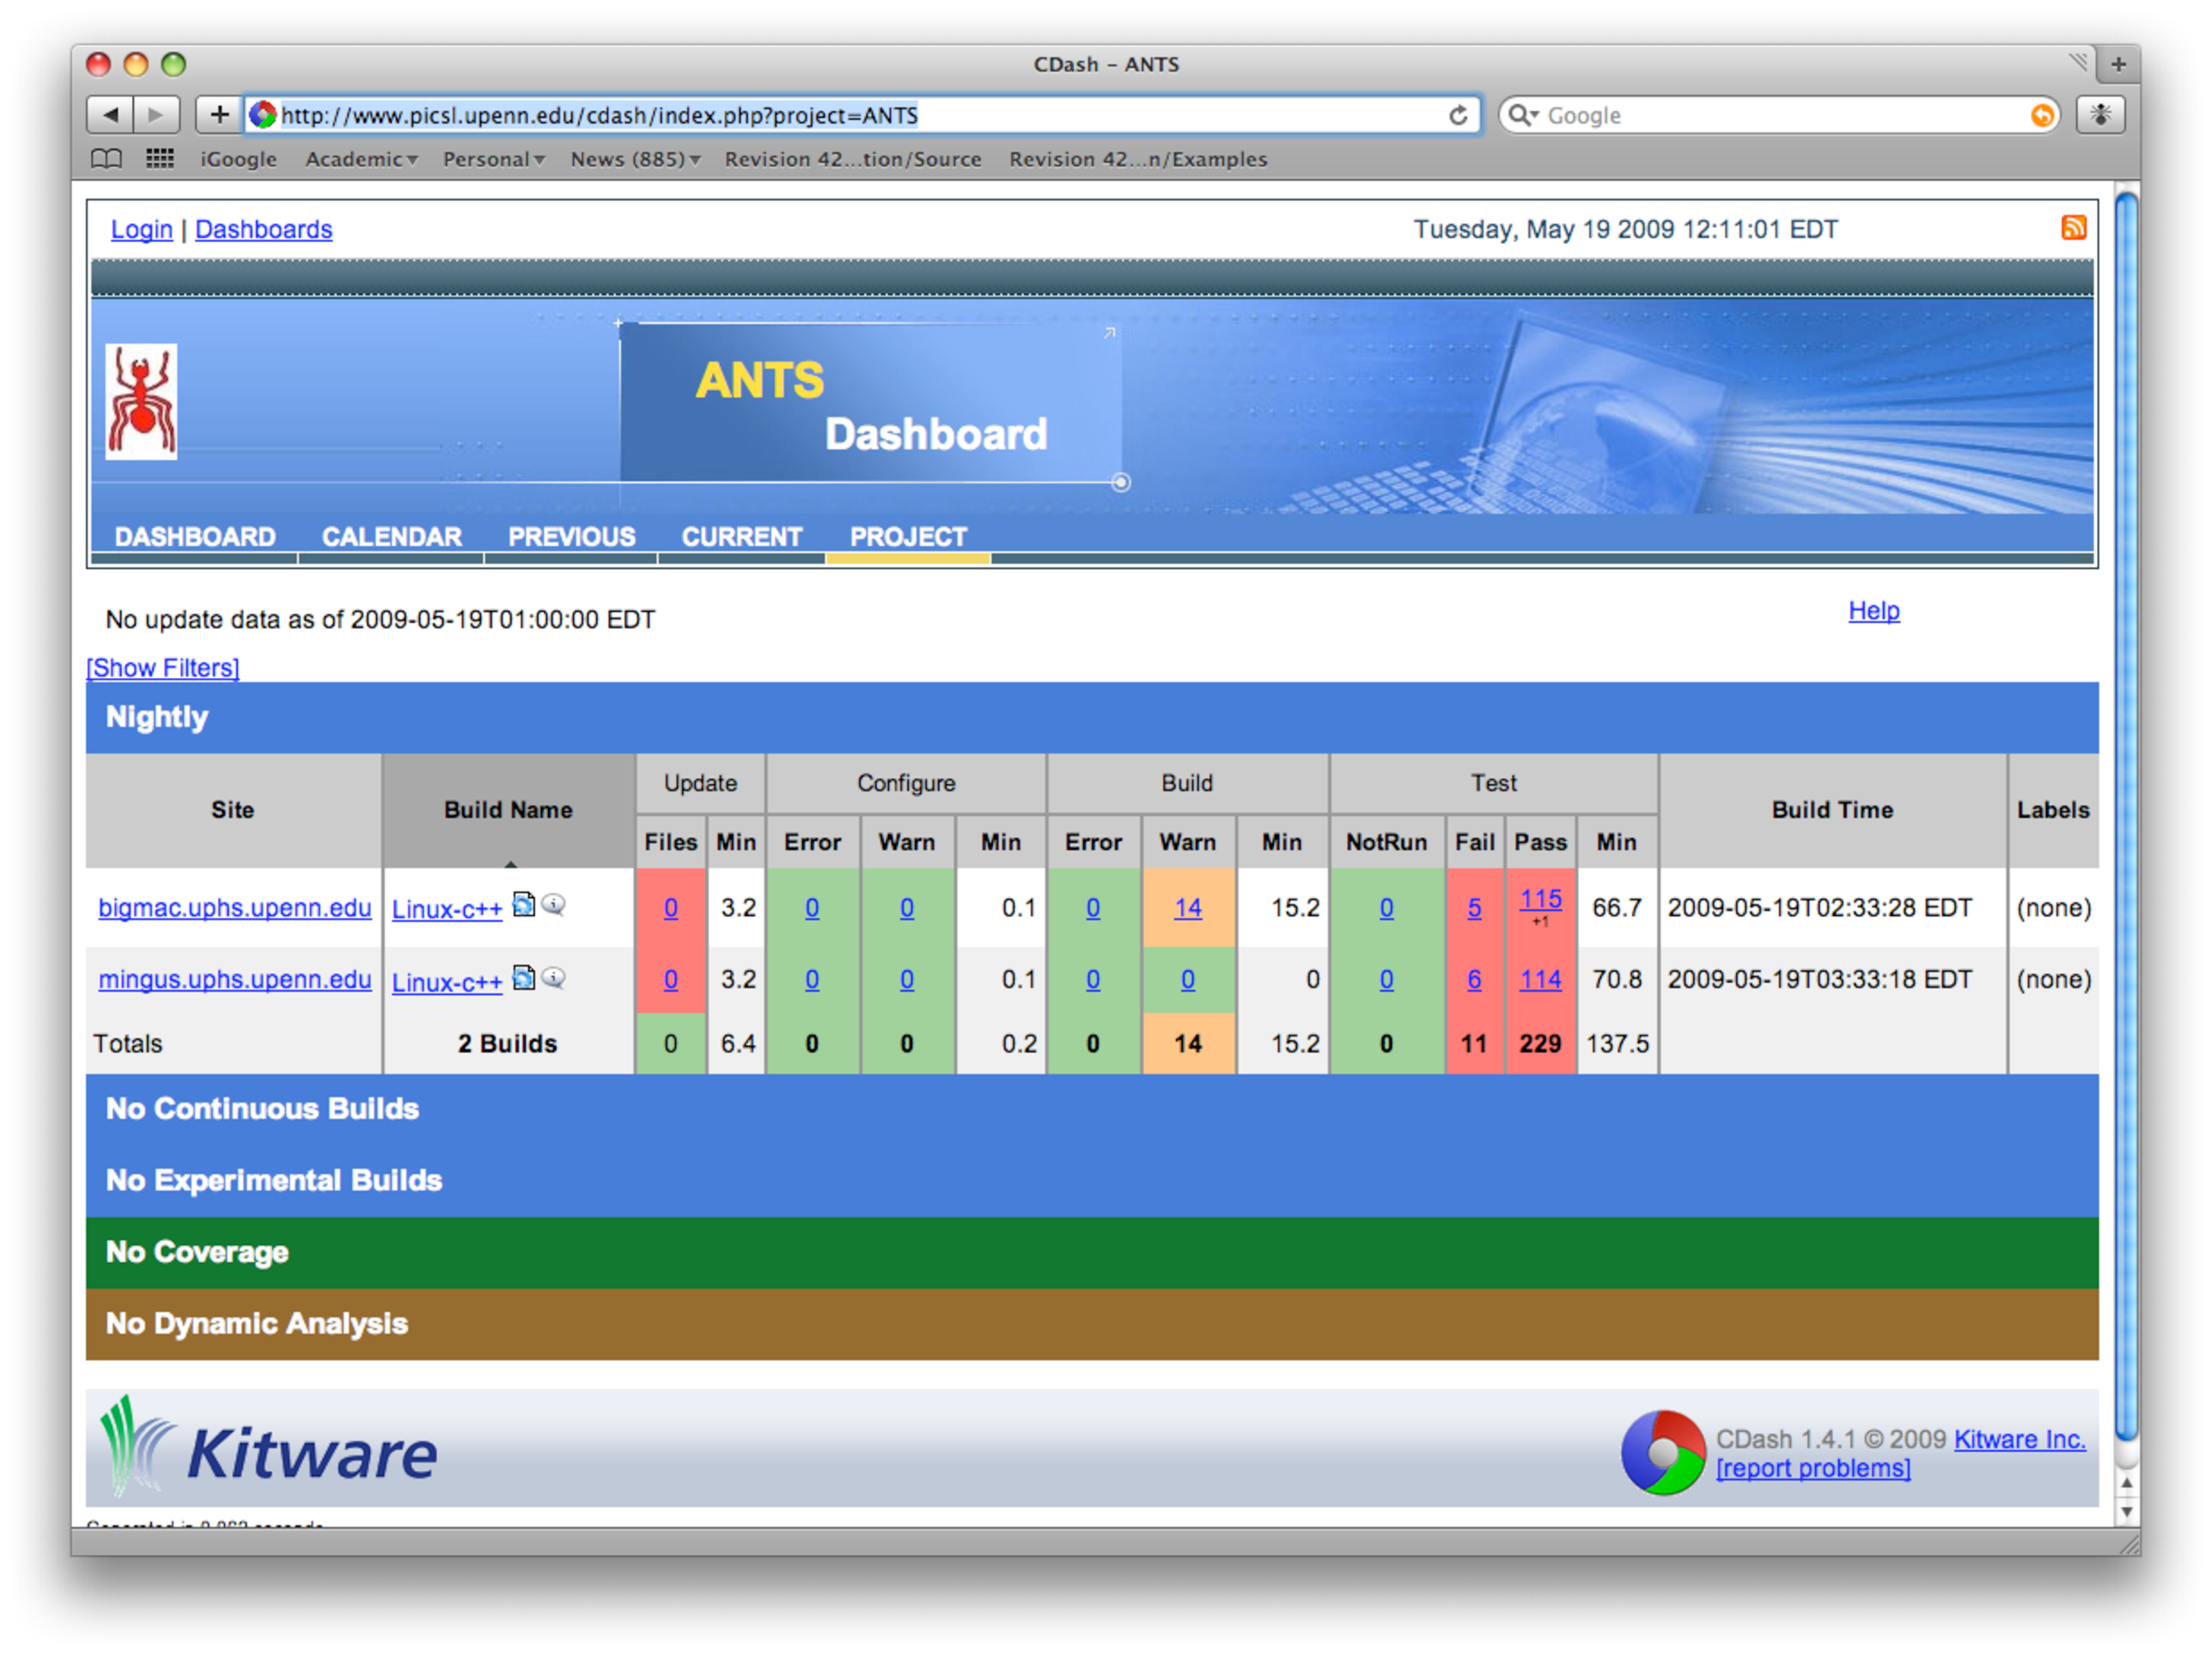
\includegraphics[width=135mm]{Figures/ANTSdashboard} 
  \end{tabular}
\caption{The ANTS dashboard, which is hosted on the PICSL website, reports daily building and testing of the ANTS software.  It also allows any user to submit their own building and testing configurations to help with debugging issues and maintenance for a variety of computing platforms. }  
\label{fig:dashboard}
\end{figure*}



Based on our experience with standard command line argument parsing packages (e.g. \verb#getopt#), we developed our own set of classes for an intuitive command line interface.  A summary of command line arguments are given in Table \ref{table:args}.  
These ANTS argument parsing classes provide an intuitive compromise between parsers where every variable requires a unique flag and strict ordering requirements on the command line.  A typical command line call to ANTS  is  given by
\begin{lstlisting}
>ANTS 3 
  --metric MSQ[fixedImage.nii,movingImage.nii,0.75] 
  --metric PSE[fixedPoints.vtk,movingPoints.vtk,0.25] 
  --transformation Exp[0.75] 
  --regularization Gauss[3.0,0.5]
  --iterations 50x20x10x5 
  --output-naming results.nii
\end{lstlisting}
The correspondence between the ANTS command line specification and the image normalization formulation with labeled point-sets $X$ and $Y$ illustrates the motivation for our command line interface,
\begin{align}
  \Pi(&\mathcal{I},\mathcal{J},X,Y,\phi) \nonumber \\ 
     =& \underbrace{\int_0^1 ||L\boldsymbol{v}||dt}_{\texttt{-t Exp[}\cdot \texttt{]},\texttt{ -r Gauss[}\cdot\texttt{,}\cdot\texttt{]}}  + \underbrace{\lambda_1\int_{\Omega} || \mathcal{I} \circ \phi(\mathbf{x},t) - \mathcal{J}  || d\Omega}_{\texttt{-t Exp[}\cdot \texttt{]},\texttt{ -m MSQ[}\mathcal{J}\texttt{,}\mathcal{I}\texttt{,}\lambda_1\texttt{]}} \nonumber \\
&+\underbrace{\frac{\lambda_2 }{|Y|}\sum_{i=1}^{|Y|} \left\|y_i - \frac{1}{|X|} \sum_{j = 1}^{|X|} G(y_i; x_j, \sigma_X) x_j\right\|^2}_{\texttt{-m PSE[}Y\texttt{,}X\texttt{,}\lambda_2\texttt{]}}.
\end{align}

In Table \ref{table:args} we give a brief summary of the arguments available for the normalizations offered by the ANTS package.  This includes the corresponding variable specification.  More information can be found on the ANTS website.  

\begin{table*}
  \centering
    \begin{tabular}{c c c c c}
   {\bf } & {\bf Argument} & {\bf Flag} & {\bf Variables}  & {\bf Sample Parameters}\\
    \toprule
    \multirow{3}*{\bf Linear}
    & Iterations & \verb#--linear-iterations# & {} & $N_1$\verb#x#$N_2$\verb#x#$N_3$\verb#x#\ldots \\ 
    & Similarity & \verb#--linear-metric# & \verb#MI,MSQ# & \verb#[#$N_{bins}$,$N_{samples}$\verb#]# \\ 
    {} & Affine or Rigid &  \verb#--do-rigid# & {} & \verb#0# \\
    \cmidrule(l){2-5}
    \multirow{5}*{\bf Deform.}
    & Image Similarity & \verb#--metric,-m# & \verb#MI,CC,PR,MSQ# & \verb#[#$\mathcal{I},\mathcal{J}$,\verb#radius]# \\
    & Point-Set Similarity & \verb#--metric,-m# & \verb#PSE,JHCT# & \verb#[#$\mathcal{I},\mathcal{J},X,Y$\verb#]# \\
    {} & Iterations/Level & \verb#--iterations,-i# & {} & $N_1$\verb#x#$N_2$\verb#x#$N_3$\verb#x#\ldots \\ 
    {} & Regularization &  \verb#--regularization,-r# & \verb#Gauss,DMFFD# & \verb#[#$\sigma^2_{gradient}$,$\sigma^2_{total}$\verb#]#, \verb#[1x1,3x3]#\\
    {} & Transformation & \verb#--transformation,-t# & \verb#Elast,SyN,Exp# & \verb#[#$\Delta_{gradient}$\verb#]# \\
    \cmidrule(l){2-5}
    \multirow{2}*{\bf Misc.}
    & Histogram Match $\mathcal{I},\mathcal{J}$ & \verb#--use-histogram-matching# & {}  & \verb#1# \\
    {} & NN Interpolation & \verb#--use-NN# & {} & \verb#0#\\
    {} & Mask Image &  \verb#--mask,-x# & {} & \verb#mask.nii# \\
    {} & Output Naming     & \verb#--output-naming,-o# & {} & \verb#filename.nii# \\
    \bottomrule
    \end{tabular}
  \caption{The various flags and variables for a variety of image registration possibilities.   Additional information can be found on the ANTS website \cite{ANTS2009}. }
  \label{table:args}
\end{table*}    

\section{Experimental Evaluation}

There are many avenues for exploration of the various components of ANTS.  However, due to space constraints, we limit experimental analysis within this paper to an extension of the normalization assessment carried out by \cite{Klein2009}.  As previously mentioned, this large-scale assessment encompassed evaluation of 14 popular registration algorithms which were optimized, in terms of their parameters, by their respective authors before a thorough brain image normalization study.  Although the Greedy SyN algorithm, outlined in an earlier section, was consistently one of the top two performers in Klein's study, for the benefit of the users of ANTS, we explore the other transformation model possibilities within ANTS and compare them with Greedy SyN.  In terms of data, we utilize the NA0 evaluation database of the Non-Rigid Image Registration Evaluation Project (NIREP) for future comparison with evaluation studies that have been proposed by the NIREP initiative.%
\footnote{http://www.nirep.org/
}

As outlined in the introduction, in addition to the transformation, the optimization strategy and similarity metric form the image normalization scheme.  Since our optimization strategy is limited to gradient descent, experimental analysis includes an exploration of optimal gradient steps within a sensible window where the steps are scaled according to the voxel spacing.  In terms of similarity metric, we limit exploration to cross-correlation while varying the radius within reasonable values.    Other metrics were not explored since the labeled brain images entail a simple intensity relationship between image pairs obviating the need for similarity metrics for more complex intensity relationships (e.g. MI) in addition to the fact that the consistently top two performers in \cite{Klein2009} used cross-correlation.

Briefly, two experiments were performed.  The first experiment consisted of a more extensive parameter search over both the transformation model space and the cross-correlation metric radius using the exhaustive pairwise combination of the eight 2-D images illustrated in Figure \ref{fig:phantoms}.  Based on the results of the first experiment, the parameter space was pruned and subsequently used for the registrations performed during the second experiment involving 10 randomly selected image pairs from the 16 labeled NA0 NIREP brain images.

\subsection{2-D Simulated Image Normalization Evaluation}

Eight simulated 2-D images were created to model the types of deformations one would encounter in brain image normalization.  Each image was created with isotropic spacing and of size $102\times95$.  The foreground of each image was comprised of two labels representing the white matter and grey matter.  Since the 2-D simulated image experiments were used to prune the transformation model space (and not the image similarity metric space) the foreground intensities were not created to model the intensity variation normally seen in the grey/white matter.  Note that these images are distributed with the ANTS open source package.

\begin{figure}
\centering
  \begin{tabular}{c}
      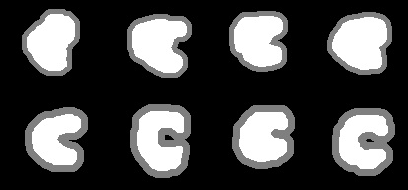
\includegraphics[width=85mm]{Figures/phantomwmgm} 
  \end{tabular}
\caption{The eight 2-D simulated images used for the initial parameter search.  These images  are available with the ANTS source distribution.}  
\label{fig:phantoms}
\end{figure}

\subsection{3-D NIREP Brain Image Normalization Evaluation}

The Non-Rigid Image Registration Project is a large-scale evaluation resource for deformable registration algorithms headed by Gary Christensen at the University of Iowa.  In addition to the development and distribution of the necessary software tools for algorithmic validation, this project includes the distribution of appropriate image data and corresponding segmentations.   One such database that has been made available is referred to as the ``NA0'' database consisting of 16 MR image volumes of normal adult human volunteers.  A brief demographic sketch of the NA0 database is as follows:  8 males with mean age of 32.5 $\pm$ 8.4 years (range of 25 to 48 years) and  8 females with mean age of 29.8 $\pm$ 5.8 years (range of 24 to 41).  

Following acquisition, each image was resampled and padded to isotropic voxel spacing of $0.7\times0.7\times0.7$ mm$^3$ and total size of $256 \times 300 \times 256$ voxels.
The cortex of each of the 16 MR image volumes was segmented into 32 regions \cite{Allen2002,Allen2003} using Brainvox which were later refined using manual editing.  

\begin{figure}
\centering
  \begin{tabular}{cc}
      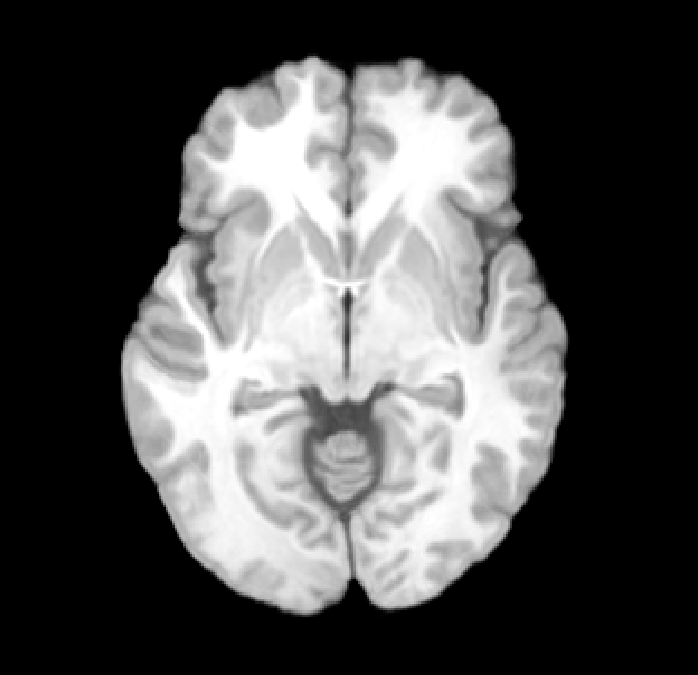
\includegraphics[width=40mm]{Figures/na01x_axial.png} &
      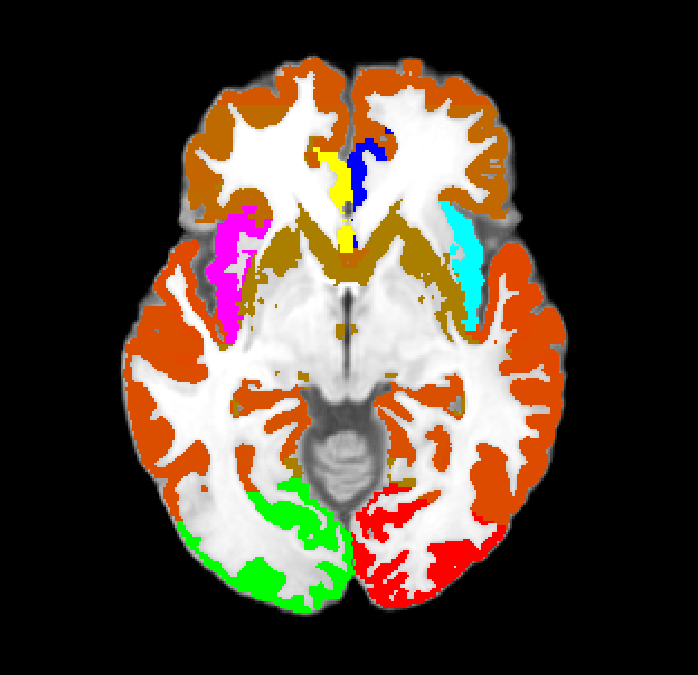
\includegraphics[width=40mm]{Figures/na01x_axial_labels.png} \\
      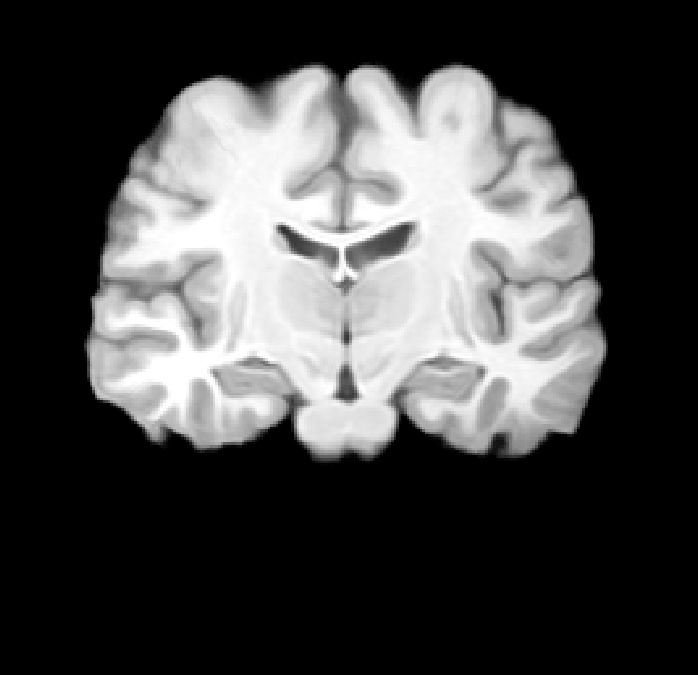
\includegraphics[width=40mm]{Figures/na01x_coronal.png} &
      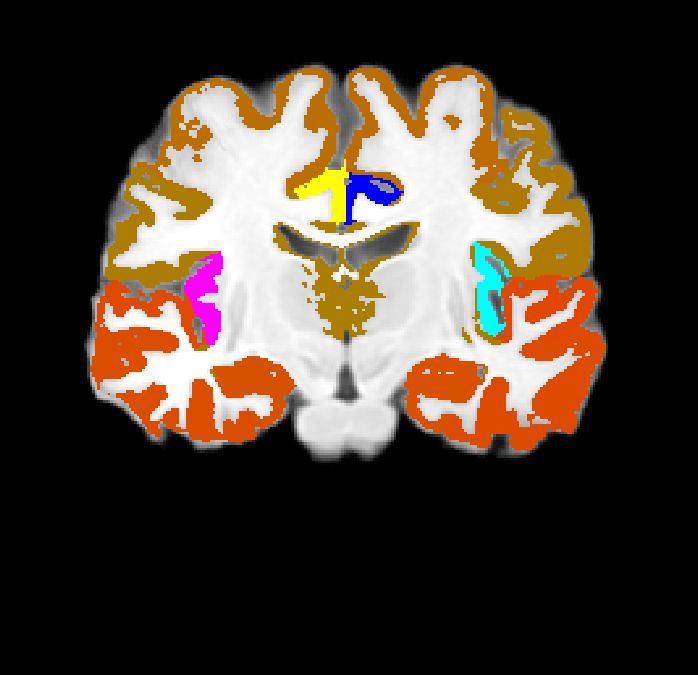
\includegraphics[width=40mm]{Figures/na01x_coronal_labels.png} \\
      \reflectbox{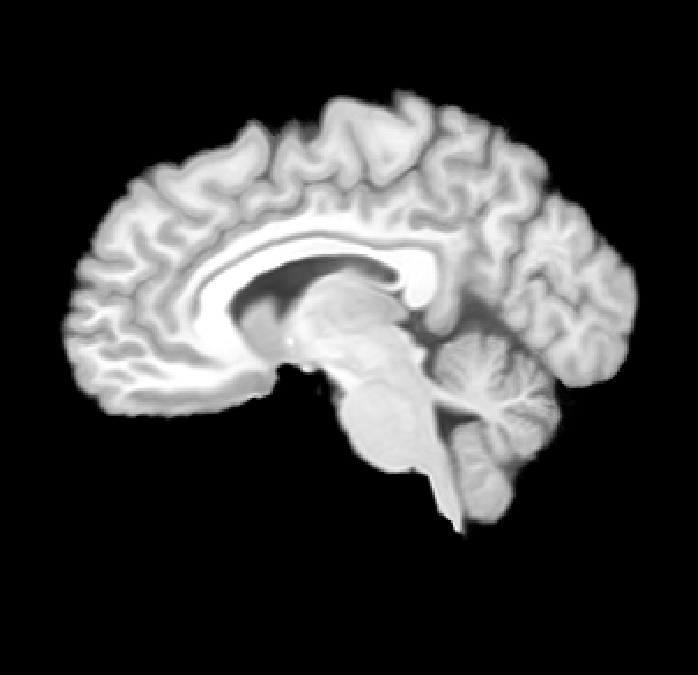
\includegraphics[width=40mm]{Figures/na01x_sagittal.png}} &
      \reflectbox{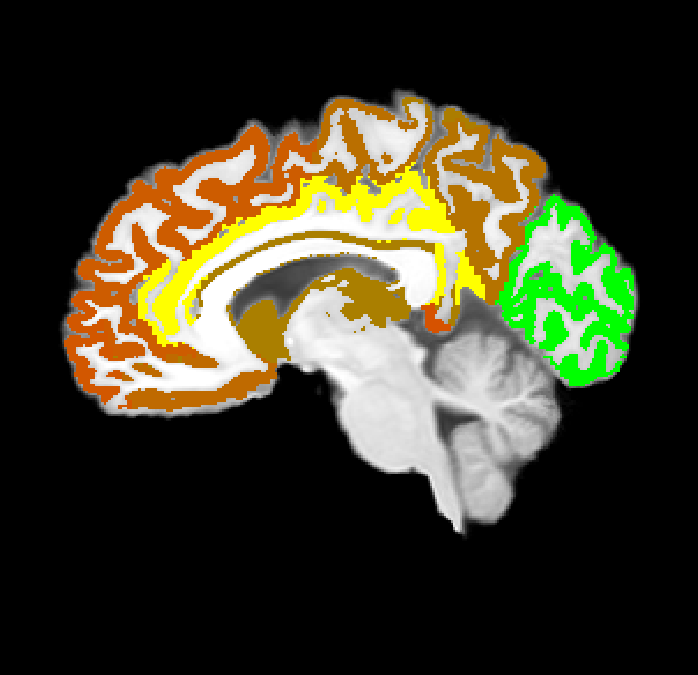
\includegraphics[width=40mm]{Figures/na01x_sagittal_labels.png}} \\
  \end{tabular}
\caption{Canonical image views of NA01 image from the NIREP data base (left column) and the corresponding segmentations (right column).  }  
\label{fig:na01x}
\end{figure}

\section{Discussion}

% use section* for acknowledgement
\section*{Acknowledgment}
ANTS is supported by Grant 1R01EB006266-01 from the National Institute Of Biomedical Imaging and Bioengineering and administered through the UCLA Center for Computational Biology.
% optional entry into table of contents (if used)
%\addcontentsline{toc}{section}{Acknowledgment}
%The authors would like to thank...

% trigger a \newpage just before the given reference
% number - used to balance the columns on the last page
% adjust value as needed - may need to be readjusted if
% the document is modified later
%\IEEEtriggeratref{8}
% The "triggered" command can be changed if desired:
%\IEEEtriggercmd{\enlargethispage{-5in}}

% references section
% NOTE: BibTeX documentation can be easily obtained at:
% http://www.ctan.org/tex-archive/biblio/bibtex/contrib/doc/

% can use a bibliography generated by BibTeX as a .bbl file
% standard IEEE bibliography style from:
% http://www.ctan.org/tex-archive/macros/latex/contrib/supported/IEEEtran/bibtex
%\bibliographystyle{IEEEtran.bst}
% argument is your BibTeX string definitions and bibliography database(s)
%\bibliography{IEEEabrv,../bib/paper}
%
% <OR> manually copy in the resultant .bbl file
% set second argument of \begin to the number of references
% (used to reserve space for the reference number labels box)

\bibliographystyle{IEEEtran.bst}
\bibliography{./references.bib}

\end{document}



